\section{Deployment view}
\begin{figure}[h]
    \centering
    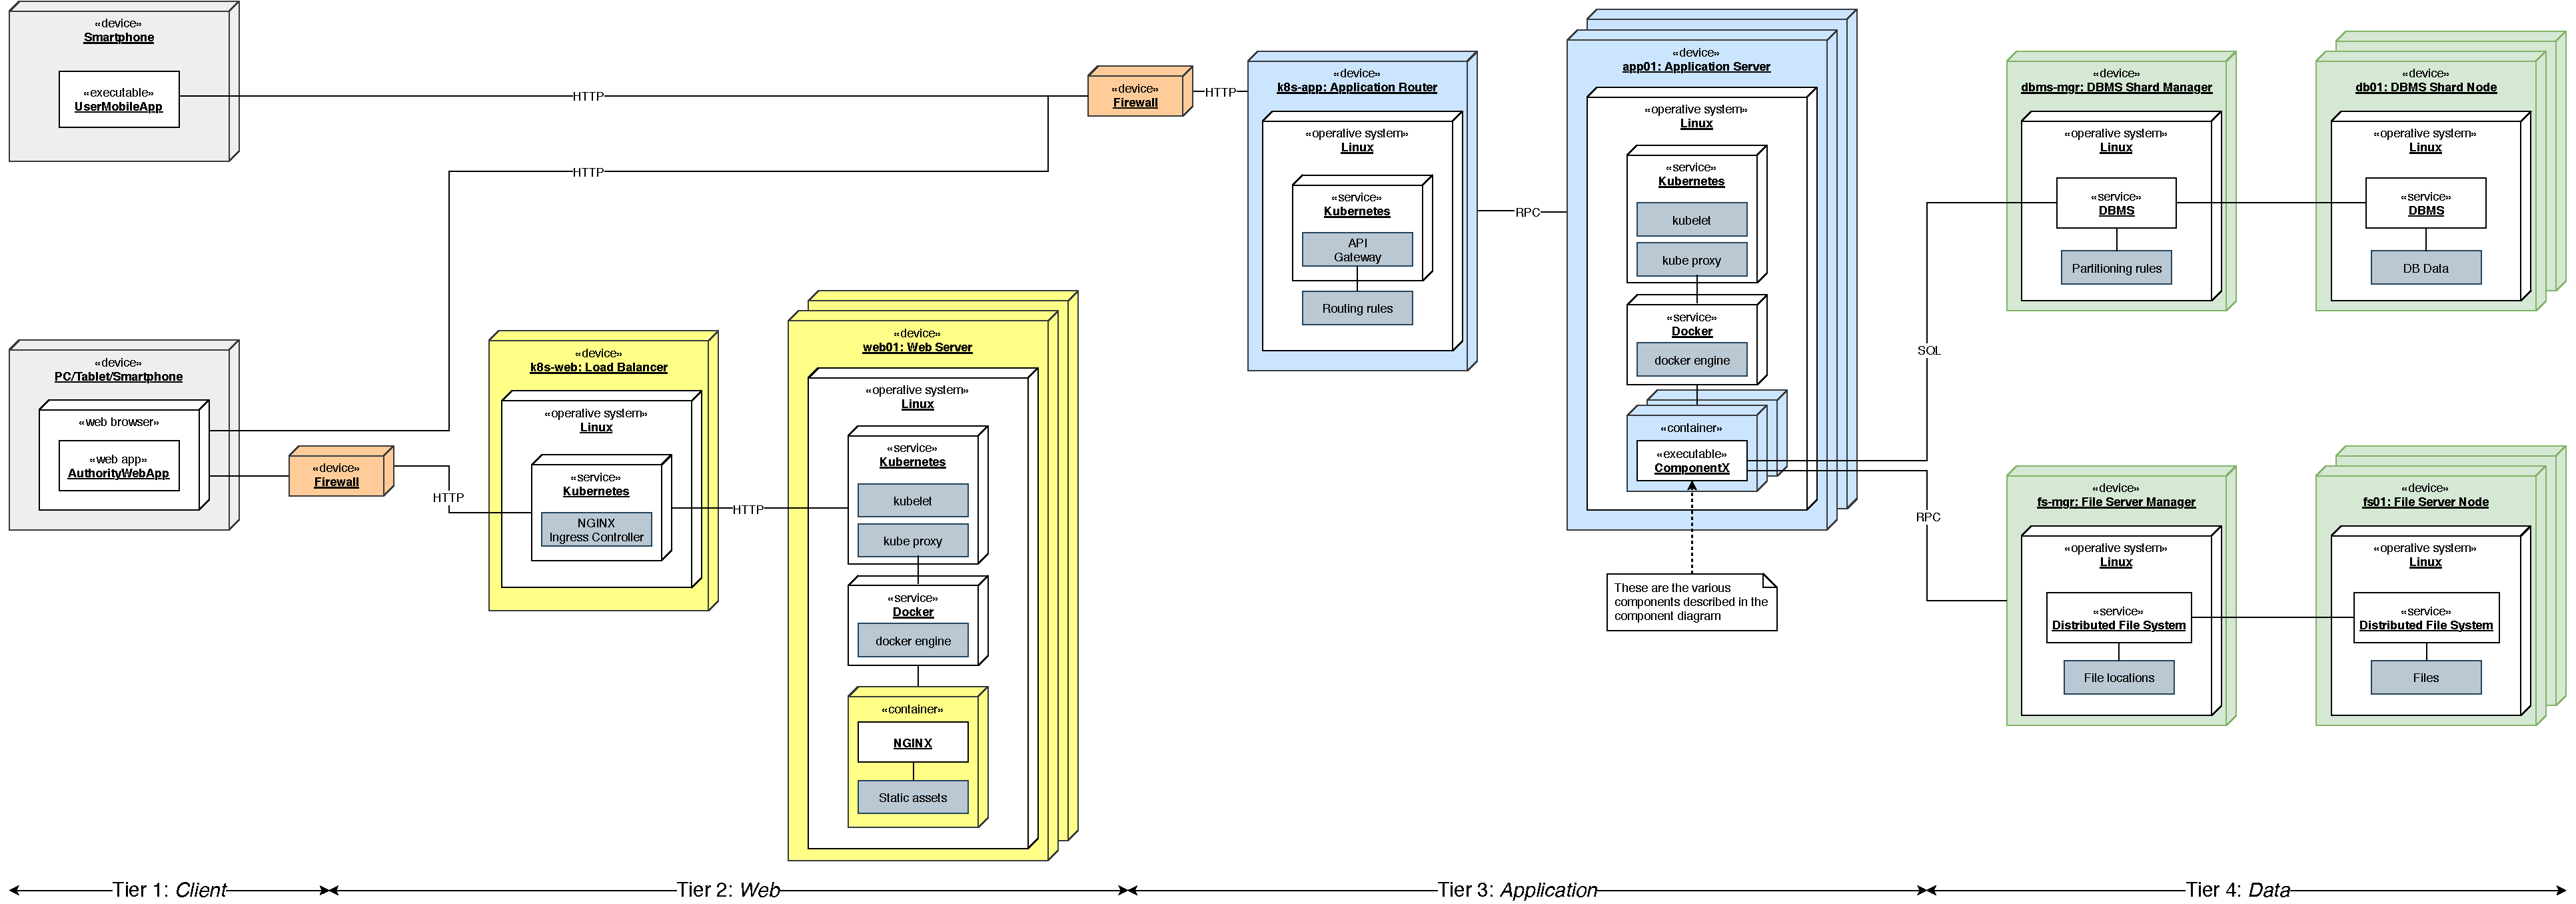
\includegraphics[width=\textwidth]{dd_deployment.pdf}
    \caption{Deployment diagram}
    \label{fig:depolyment_diagram}
\end{figure}

The diagram in figure~\vref{fig:depolyment_diagram} shows the deployment plan
for the various components of the system. External components (such and the DMV
and municipality systems) are not shown, since they are already built and
deployed, and they can just be accessed from the internet.
The diagram shows the \emph{physical devices} in which the components will run,
the \emph{communication channels} between the components and their
\emph{software environment}.
The system is split into \emph{four tiers}, the last three heavily relying on
replication to achieve scalability and fault tolerance.

\begin{description}
    \item[Client tier] It is composed by the end-user interfaces:
    the \emph{mobile application} for the citizen and the \emph{web application}
    for the authority.
    The first one must be developed for both Android and iOS, as required in
    the RASD, and communicates directly to the application tier by using
    HTTP (specifically a REST API).

    The website, on the other hand, only requires a web browser to be used,
    and therefore it can run on PCs, as well as tablets and smartphones,
    although the focus should be mainly on PCs.
    It interacts with the web tier through HTTP (to request static assets)
    and to the application tier also through HTTP, using the REST API.
    \item[Web tier] This tier contains the \emph{WebServer} component,
    represented by NGINX, which has been chosen for its reliability and
    performance for static serving.
    NGINX actually runs inside a Docker container, which also contains the HTML,
    CSS and JS files to be served. The containers are orchestrated by
    \emph{Kubernetes}, which takes care of auto-scaling, load balancing, image
    and configuration deployment thanks to the \emph{NGINX Ingress Controller}.
    There is a single node (\emph{k8s-web}) that acts as a Kubernetes manager.
    It is worth pointing out that, since NGINX already uses internal workers,
    there are no advantages on deploying more than one container to each
    replicated node.
    \item[Application tier] This tier is responsible for the components that
    implement the business logic of the system, see section~%
    \ref{sec:component_view} for more details on them.
    As in tier 2, we rely on Kubernetes and Docker for replication.
    Here the Kubernetes manager (\emph{k8s-app}) implements the \emph{Router}
    component through an API gateway module.
    The role of this module is to accept REST requests and route them to
    the correct container as remote procedure calls (RPCs).
    Each container runs a specific application component and they communicate
    between themselves through RPC. Differently from tier 2, here it makes sense
    to run multiple containers on the same node.
    \item[Data tier] This tier contains the components responsible for
    persistently storing data: the database and the file server.
    The database component is implemented as a Relational Database Management
    System (RDBMS), to which application components send SQL queries.
    Since the data stored in the DB will most likely exceed the capacity of a
    single node over time, it is horizontally partitioned over multiple nodes
    using \emph{database sharding} (see section~\ref{subsec:db_sharding}):
    there is a single node that acts as the transaction manager, while the
    actual data resides on the \emph{shard nodes}.

    The consideration made for the DB also holds for the file server: at one
    point the collected images will exceed the capacity of a single node.
    In the same way the files are partitioned over multiple nodes and there is
    a single manager that keeps the mapping between the file names and their
    actual locations. The communication with the application tier relies on RPC.
    
    In this way the application tier only sees one entrypoint for the DBMS and
    one for the file server, which hide the internal replication.
\end{description}

\noindent
For more details on the design choices, in particular how data is partitioned
between nodes (and also under which assumptions),
see~\ref{sec:arch_styles_patterns}.
